\section{Exercises}

%__________________
\subsection{Variability in estimates}

% 1

\eoce{\qt{Identify the parameter, Part I} For each of the following situations, state whether the parameter of interest is a mean or a proportion. It may be helpful to examine whether individual responses are numerical or categorical.
\begin{parts}
\item In a survey, one hundred college students are asked how many hours per week they spend on the Internet.
\item In a survey, one hundred college students are asked: ``What percentage of the time you spend on the Internet is part of your course work?"
\item In a survey, one hundred college students are asked whether or not they cited information from Wikipedia in their papers.
\item In a survey, one hundred college students are asked what percentage of their total weekly spending is on alcoholic beverages.
\item In a sample of one hundred recent college graduates, it is found that 85 percent expect to get a job within one year of their graduation date.
\end{parts}
}{}

% 2

\eoce{\qt{Identify the parameter, Part II} For each of the following situations, state whether the parameter of interest is a mean or a proportion. 
\begin{parts}
\item A poll shows that 64\% of Americans personally worry a great deal about federal spending and the budget deficit.
\item A survey reports that local TV news has shown a 17\% increase in revenue between 2009 and 2011 while newspaper revenues decreased by 6.4\% during this time period.
\item In a survey, high school and college students are asked whether or not they use geolocation services on their smart phones.
\item In a survey, internet users are asked whether or not they purchased any Groupon coupons.
\item In a survey, internet users are asked how many Groupon coupons they purchased over the last year.
\end{parts}
}{}

% 3

\eoce{\qt{College credits} \label{credits} A college counselor is interested in estimating how many credits a student typically enrolls in each semester. The counselor decides to randomly sample 100 students by using the registrar's database of students. The histogram below shows the distribution of the number of credits taken by these students. Sample statistics for this distribution are also provided.\\
\begin{minipage}[c]{0.7\textwidth}
\begin{center}
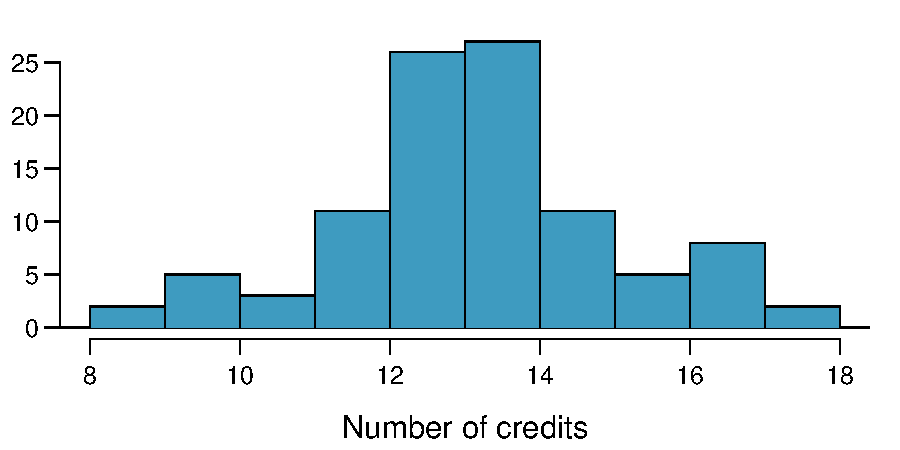
\includegraphics[width=96mm]{ch_inference_foundations_oi_biostat/figures/eoce/credits/credits}
\end{center}
\end{minipage}
\begin{minipage}[c]{0.3\textwidth}
\begin{center}
\begin{tabular}{l|r l}
Min		& 8 \\
Q1		& 13 \\
Median	& 14 \\
Mean	& 13.65 \\
SD		& 1.91 \\
Q3		& 15 \\
Max		& 18 \\
\end{tabular}
\end{center}
\end{minipage}
\begin{parts}
\item What is the point estimate for the average number of credits taken per semester by students at this college? What about the median? \textB{\newpage}
\item What is the point estimate for the standard deviation of the number of credits taken per semester by students at this college? What about the IQR?
\item Is a load of 16 credits unusually high for this college? What about 18 credits? Explain your reasoning. \textit{Hint:} Observations farther than two standard deviations from the mean are usually considered to be unusual.
\item The college counselor takes another random sample of 100 students and this time finds a sample mean of 14.02 units. Should she be surprised that this sample statistic is slightly different than the one from the original sample? Explain your reasoning.
\item The sample means given above are point estimates for the mean number of credits taken by all students at that college. What measures do we use to quantify the variability of this estimate? Compute this quantity using the data from the original sample.\end{parts}
}{}

% 4

\eoce{\qt{Heights of adults} \label{heights} Researchers studying anthropometry collected body girth measurements and skeletal diameter measurements, as well as age, weight, height and gender, for 507 physically active individuals. The histogram below shows the sample distribution of heights in centimeters. \footfullcite{Heinz:2003} \\
\begin{minipage}[c]{0.7\textwidth}
\begin{center}
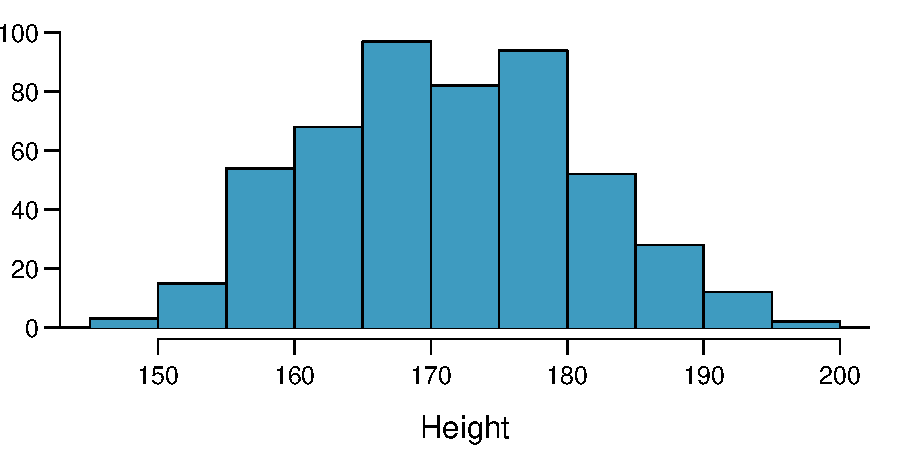
\includegraphics[width=85mm]{ch_inference_foundations_oi_biostat/figures/eoce/bdims/bdims_heights}
\end{center}
\end{minipage}
\begin{minipage}[c]{0.3\textwidth}
\begin{center}
\begin{tabular}{l|r l}
Min		& 147.2 \\
Q1		& 163.8 \\
Median	& 170.3 \\
Mean	& 171.1 \\
SD		&  9.4 \\
Q3		& 177.8 \\
Max		& 198.1 \\
\end{tabular}
\end{center}
\end{minipage}
\begin{parts}
\item What is the point estimate for the average height of active individuals? What about the median?
\item What is the point estimate for the standard deviation of the heights of active individuals? What about the IQR?
\item Is a person who is 1m 80cm (180 cm) tall considered unusually tall? And is a person who is 1m 55cm (155cm) considered unusually short? Explain your reasoning.
\item The researchers take another random sample of physically active individuals. Would you expect the mean and the standard deviation of this new sample to be the ones given above? Explain your reasoning.
\item The sample means obtained are point estimates for the mean height of all active individuals, if the sample of individuals is equivalent to a simple random sample. What measure do we use to quantify the variability of such an estimate? Compute this quantity using the data from the original sample under the condition that the data are a simple random sample. 
\end{parts}
}{}

% 5

\eoce{\qt{Wireless routers} John is shopping for wireless routers and is overwhelmed by the number of available options. In order to get a feel for the average price, he takes a random sample of 75 routers and finds that the average price for this sample is \$75 and the standard deviation is \$25. 
\begin{parts}
\item Based on this information, how much variability should he expect to see in the mean prices of repeated samples, each containing 75 randomly selected wireless routers?
\item A consumer website claims that the average price of routers is \$80. Is a true average of \$80 consistent with John's sample?
\end{parts}
}{}

\textB{\newpage}

% 6

\eoce{\qt{Chocolate chip cookies} Students are asked to count the number of chocolate chips in 22 cookies for a class activity. They found that the cookies on average had 14.77 chocolate chips with a standard deviation of 4.37 chocolate chips.
\begin{parts}
\item Based on this information, about how much variability should they expect to see in the mean number of chocolate chips in random samples of 22 chocolate chip cookies?
\item The packaging for these cookies claims that there are at least 20 chocolate chips per cookie. One student thinks this number is unreasonably high since the average they found is much lower. Another student claims the difference might be due to chance. What do you think?
\end{parts}
}{}


%__________________
\subsection{Confidence intervals}

% 7

\eoce{\qt{Relaxing after work} \label{relax} The General Social Survey (GSS) is a sociological survey used to collect data on demographic characteristics and attitudes of residents of the United States. In 2010, the survey collected responses from 1,154 US residents. The survey is conducted face-to-face with an in-person interview of a randomly-selected sample of adults. One of the questions on the survey is ``After an average work day, about how many hours do you have to relax or pursue activities that you enjoy?" A 95\% confidence interval from the 2010 GSS survey is 3.53 to 3.83 hours.\footfullcite{data:gss:2010}
\begin{parts}
\item Interpret this interval in the context of the data.
\item What does a 95\% confidence level mean in this context?
%\item If the researchers who conducted this survey wanted to report a confidence interval with a smaller margin of error based on the same sample of 1,154 Americans, would the confidence level be larger, smaller, or about the same?
\item Suppose the researchers think a 90\% confidence level would be more appropriate for this interval. Will this new interval be smaller or larger than the 95\% confidence interval? Assume the standard deviation has remained constant since 2010.
\end{parts}
}{}

% 8

\eoce{\qt{Mental health} Another question on the General Social Survey introduced in Exercise~\ref{relax} is ``For how many days during the past 30 days was your mental health, which includes stress, depression, and problems with emotions, not good?" Based on responses from 1,151 US residents, the survey reported a 95\% confidence interval of 3.40 to 4.24 days in 2010.
\begin{parts}
\item Interpret this interval in context of the data.
\item What does a 95\% confidence level mean in this context?
\item Suppose the researchers think a 99\% confidence level would be more appropriate for this interval. Will this new interval be smaller or larger than the 95\% confidence interval?
\item If a new survey asking the same questions was to be done with 500 Americans, would the standard error of the estimate be larger, smaller, or about the same. Assume the standard deviation has remained constant since 2010.
\end{parts}
}{}

% 9

\eoce{\qt{Width of a confidence interval} Earlier in Chapter~\ref{foundationsForInference}, we calculated the 99\% confidence interval for the average age of runners in the 2012 Cherry Blossom Run as (32.7, 37.4) based on a sample of 100 runners. How could we decrease the width of this interval without losing confidence?
}{}

% 10

\eoce{\qt{Confidence levels} If a higher confidence level means that we are more confident about the number we are reporting, why don't we always report a confidence interval with the highest possible confidence level?
}{}

\textB{\newpage}

% 11

\eoce{\qt{Waiting at an ER, Part I} \label{ERwait} A hospital administrator hoping to improve wait times decides to estimate the average emergency room waiting time at her hospital. She collects a simple random sample of 64 patients and determines the time (in minutes) between when they checked in to the ER until they were first seen by a doctor. A 95\% confidence interval based on this sample is (128 minutes, 147 minutes), which is based on the normal model for the mean. Determine whether the following statements are true or false, and explain your reasoning for those statements you identify as false.
\begin{parts}

\item This confidence interval is not valid since we do not know if the population distribution of the ER wait times is nearly normal.

\item We are 95\% confident that the average waiting time of these 64 emergency room patients is between 128 and 147 minutes.

\item We are 95\% confident that the average waiting time of all patients at this hospital's emergency room is between 128 and 147 minutes.

\item 95\% of such random samples would have a sample mean between 128 and 147 minutes.

\item A 99\% confidence interval would be narrower than the 95\% confidence interval since we need to be more sure of our estimate.

\item The margin of error is 9.5 and the sample mean is 137.5.

\item In order to decrease the margin of error of a 95\% confidence interval to half of what it is now, we would need to double the sample size.

\end{parts}
}{}

% 12

\eoce{\qt{Thanksgiving spending, Part I} \label{holidaySpending} The 2009 holiday retail season, which kicked off on November 27, 2009 (the day after Thanksgiving), had been marked by somewhat lower self-reported consumer spending than was seen during the comparable period in 2008. To get an estimate of consumer spending, 436 randomly sampled American adults were surveyed. Daily consumer spending for the six-day period after Thanksgiving, spanning the Black Friday weekend and Cyber Monday, averaged \$84.71. A 95\% confidence interval based on this sample is (\$80.31, \$89.11). Determine whether the following statements are true or false, and explain your reasoning.\vspaceB{-3mm}
\begin{center}
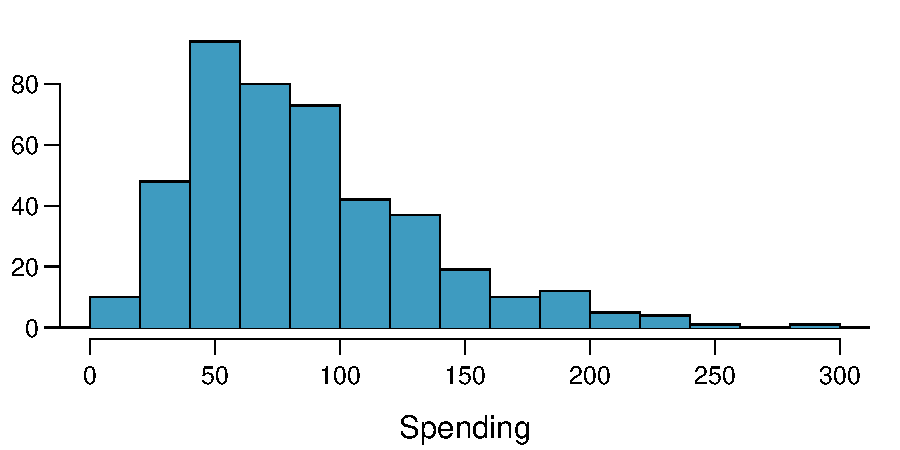
\includegraphics[width=0.7\textwidth]{ch_inference_foundations_oi_biostat/figures/eoce/tgSpending/tgSpending}
\end{center}\vspaceB{-2mm}
\begin{parts}
\item We are 95\% confident that the average spending of these 436 American adults is between \$80.31 and \$89.11.
\item This confidence interval is not valid since the distribution of spending in the sample is right skewed.
\item 95\% of such random samples would have a sample mean between \$80.31 and \$89.11.
\item We are 95\% confident that the average spending of all American adults is between \$80.31 and \$89.11.
\item A 90\% confidence interval would be narrower than the 95\% confidence interval.
\item In order to decrease the margin of error of a 95\% confidence interval to a third of what it is now, we would need to use a sample 3 times larger.
\item The margin of error for the reported interval is 4.4.
\end{parts}
}{}

% 13

\eoce{\qt{Exclusive relationships} A survey was conducted on 203 undergraduates from Duke University who took an introductory statistics course in Spring 2012. Among many other questions, this survey asked them about the number of exclusive relationships they have been in. The histogram below shows the distribution of the data from this sample. The sample average is 3.2 with a standard deviation of 1.97.
\begin{center}
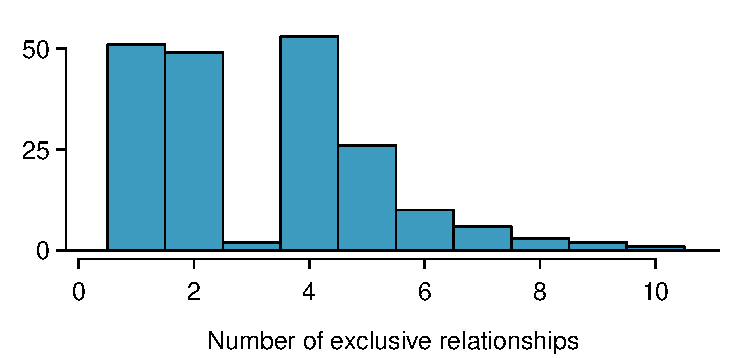
\includegraphics[width=0.65\textwidth]{ch_inference_foundations_oi_biostat/figures/eoce/relationship/rel_hist}
\end{center}
Estimate the average number of exclusive relationships Duke students have been in using a 90\% confidence interval and interpret this interval in context. Check any conditions required for inference, and note any assumptions you must make as you proceed with your calculations and conclusions.
}{}

% 14

\eoce{\qt{Age at first marriage, Part I} \label{ageAtMar} The National Survey of Family Growth conducted by the Centers for Disease Control gathers information on family life, marriage and divorce, pregnancy, infertility, use of contraception, and men's and women's health. One of the variables collected on this survey is the age at first marriage. The histogram below shows the distribution of ages at first marriage of 5,534 randomly sampled women between 2006 and 2010. The average age at first marriage among these women is 23.44 with a standard deviation of 4.72.\footfullcite{data:nsfg:2010}
\begin{center}
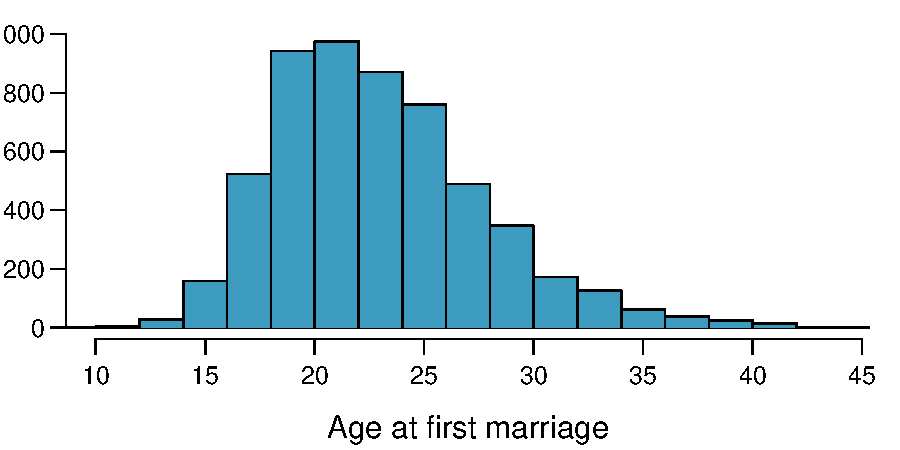
\includegraphics[width=0.7\textwidth]{ch_inference_foundations_oi_biostat/figures/eoce/ageAtMar/ageAtMar_hist}
\end{center}
Estimate the average age at first marriage of women using a 95\% confidence interval, and interpret this interval in context. Discuss any relevant assumptions.
}{}


\textB{\newpage}


%__________________
\subsection{Hypothesis testing}

% 15

\eoce{\qt{Identify hypotheses, Part I} Write the null and alternative hypotheses in words and then symbols for each of the following situations.
\begin{parts}
\item New York is known as ``the city that never sleeps". A random sample of 25 New Yorkers were asked how much sleep they get per night. Do these data provide convincing evidence that New Yorkers on average sleep less than 8 hours a night?
\item Employers at a firm are worried about the effect of March Madness, a basketball championship held each spring in the US, on employee productivity. They estimate that on a regular business day employees spend on average 15 minutes of company time checking personal email, making personal phone calls, etc. They also collect data on how much company time employees spend on such non-business activities during March Madness. They want to determine if these data provide convincing evidence that employee productivity decreases during March Madness.
\end{parts}
}{}

% 16

\eoce{\qt{Identify hypotheses, Part II} Write the null and alternative hypotheses in words and using symbols for each of the following situations.
\begin{parts}
\item Since 2008, chain restaurants in California have been required to display calorie counts of each menu item. Prior to menus displaying calorie counts, the average calorie intake of diners at a restaurant was 1100 calories. After calorie counts started to be displayed on menus, a nutritionist collected data on the number of calories consumed at this restaurant from a random sample of diners. Do these data provide convincing evidence of a difference in the average calorie intake of a diners at this restaurant?
\item Based on the performance of those who took the GRE exam between July 1, 2004 and June 30, 2007, the average Verbal Reasoning score was calculated to be 462. In 2011 the average verbal score was slightly higher. Do these data provide convincing evidence that the average GRE Verbal Reasoning score has changed since 2004? \footfullcite{webpage:GRE} 
\end{parts}
}{}

% 17

\eoce{\qt{Online communication} A study suggests that the average college student spends 2 hours per week communicating with others online. You believe that this is an underestimate and decide to collect your own sample for a hypothesis test. You randomly sample 60 students from your dorm and find that on average they spent 3.5 hours a week communicating with others online. A friend of yours, who offers to help you with the hypothesis test, comes up with the following set of hypotheses. Indicate any errors you see.\vspaceB{-2mm}
\begin{align*}
H_0&: \bar{x} < 2~hours \\
H_A&: \bar{x} > 3.5~hours
\end{align*}
}{}

% 18

\eoce{\qt{Age at first marriage, Part II} Exercise~\ref{ageAtMar} presents the results of a 2006 - 2010 survey showing that the average age of women at first marriage is 23.44. Suppose a researcher believes that this value has increased in 2012, but he would also be interested if he found a decrease. Below is how he set up his hypotheses. Indicate any errors you see.\vspaceB{-2mm}
\begin{align*}
H_0&: \bar{x} = 23.44~years~old \\
H_A&: \bar{x} > 23.44~years~old
\end{align*}
}{}

% 19

\eoce{\qt{Waiting at an ER, Part II} Exercise~\ref{ERwait} provides a 95\% confidence interval for the mean waiting time at an emergency room (ER) of (128 minutes, 147 minutes). 
\begin{parts}
\item A local newspaper claims that the average waiting time at this ER exceeds 3 hours. What do you think of this claim?
\item The Dean of Medicine at this hospital claims the average wait time is 2.2 hours. What do you think of this claim?
\item Without actually calculating the interval, determine if the claim of the Dean from part (b) would be considered reasonable based on a 99\% confidence interval?
\end{parts}
}{}

% 20

\eoce{\qt{Thanksgiving spending, Part II} Exercise~\ref{holidaySpending} provides a 95\% confidence interval for the average spending by American adults during the six-day period after Thanksgiving 2009: (\$80.31, \$89.11). 
\begin{parts}
\item A local news anchor claims that the average spending during this period in 2009 was \$100. What do you think of this claim?
\item Would the news anchor's claim be considered reasonable based on a 90\% confidence interval? Why or why not?
\end{parts}
}{}

% 21

\eoce{\qt{Ball bearings} A manufacturer claims that bearings produced by their machine last 7 hours on average under harsh conditions. A factory worker randomly samples 75 ball bearings, and records their lifespans under harsh conditions. He calculates a sample mean of 6.85 hours, and the standard deviation of the data is 1.25 working hours. The following histogram shows the distribution of the lifespans of the ball bearings in this sample. Conduct a formal hypothesis test of this claim. Make sure to check that relevant conditions are satisfied.
\begin{center}
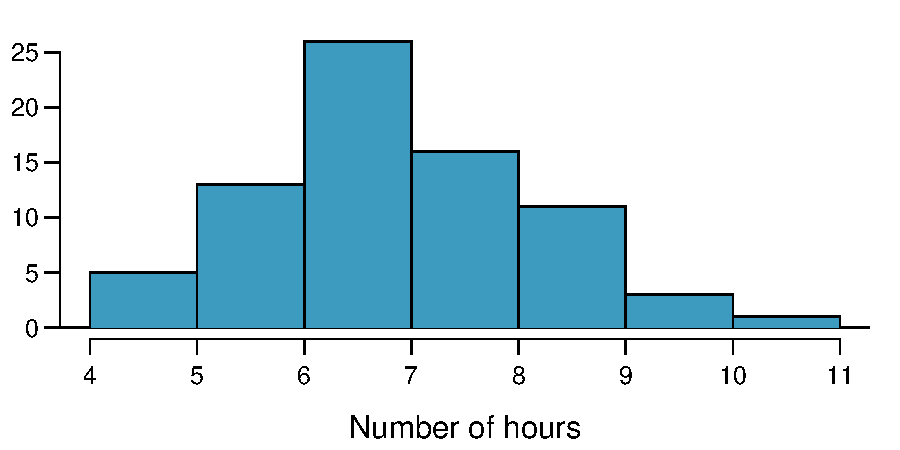
\includegraphics[width=0.6\textwidth]{ch_inference_foundations_oi_biostat/figures/eoce/ballBearing/ballBearing}
\end{center}
}{}

% 22

\eoce{\qt{Gifted children, Part I} \label{gifted} Researchers investigating characteristics of gifted children collected data from schools in a large city on a random sample of thirty-six children who were identified as gifted children soon after they reached the age of four. The following histogram shows the distribution of the ages (in months) at which these children first counted to 10 successfully. Also provided are some sample statistics.\footfullcite{Graybill:1994}

\begin{center}
\begin{minipage}[c]{0.5\textwidth}
\begin{center}
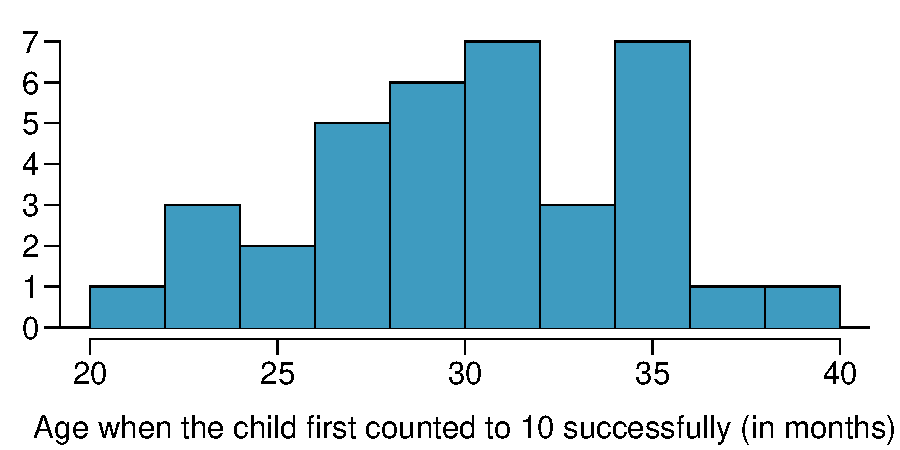
\includegraphics[width=\textwidth]{ch_inference_foundations_oi_biostat/figures/eoce/gifted/gifted_count_hist} 
\end{center}
\end{minipage}
\begin{minipage}[c]{0.1\textwidth}
\begin{tabular}{r | l}
n	& 36 \\
min	& 21 \\
mean	& 30.69 \\
sd	& 4.31 \\
max	& 39 
\end{tabular}
\end{minipage}
\end{center}

\begin{parts}
\item Are conditions for inference satisfied?
\item Suppose you read on a parenting website that children first count to 10 successfully when they are 32 months old, on average. Perform a hypothesis test to evaluate if these data provide convincing evidence that the average age at which gifted children first count to 10 successfully is different than the general average of 32 months. Use a significance level of 0.10.
\item Interpret the p-value in context of the hypothesis test and the data. 
\item Calculate a 90\% confidence interval for the average age at which gifted children first count to 10 successfully.
\item Do your results from the hypothesis test and the confidence interval agree? Explain.
\end{parts}
}{}

% 23

\eoce{\qt{Waiting at an ER, Part III} \label{ERWaitHT} The hospital administrator mentioned in Exercise~\ref{ERwait} randomly selected 64 patients and measured the time (in minutes) between when they checked in to the ER and the time they were first seen by a doctor. The average time is 137.5 minutes and the standard deviation is 39 minutes. He is getting grief from his supervisor on the basis that the wait times in the ER increased greatly from last year's average of 127 minutes. However, the administrator claims that the increase is probably just due to chance. 
\begin{parts}
\item Are conditions for inference met? Note any assumptions you must make to proceed.
\item Using a significance level of $\alpha = 0.05$, is the change in wait times statistically significant? Use a two-sided test since it seems the supervisor had to inspect the data before he suggested an increase occurred.
\item Would the conclusion of the hypothesis test change if the significance level was changed to $\alpha = 0.01$?
\end{parts}
}{}

% 24

\eoce{\qt{Gifted children, Part II} Exercise~\ref{gifted} describes a study on gifted children. In this study, along with variables on the children, the researchers also collected data on the mother's and father's IQ of the 36 randomly sampled gifted children. The histogram below shows the distribution of mother's IQ.  Also provided are some sample statistics.\\[-2mm]
\begin{minipage}[c]{0.43\textwidth}
\begin{parts}
\item Perform a hypothesis test to evaluate if these data provide convincing evidence that the average IQ of mothers of gifted children is different than the average IQ for the population at large, which is 100. Use a significance level of 0.10.
\item Calculate a 90\% confidence interval for the average IQ of mothers of gifted children.
\item Do your results from the hypothesis test and the confidence interval agree? Explain.
\end{parts}
\end{minipage}
\begin{minipage}[c]{0.56\textwidth}
\begin{center}
{\small\begin{tabular}{r | l}
n	& 36 \\
min	& 101 \\
mean	& 118.2 \\
sd	& 6.5 \\
max	& 131 
\end{tabular}} \\
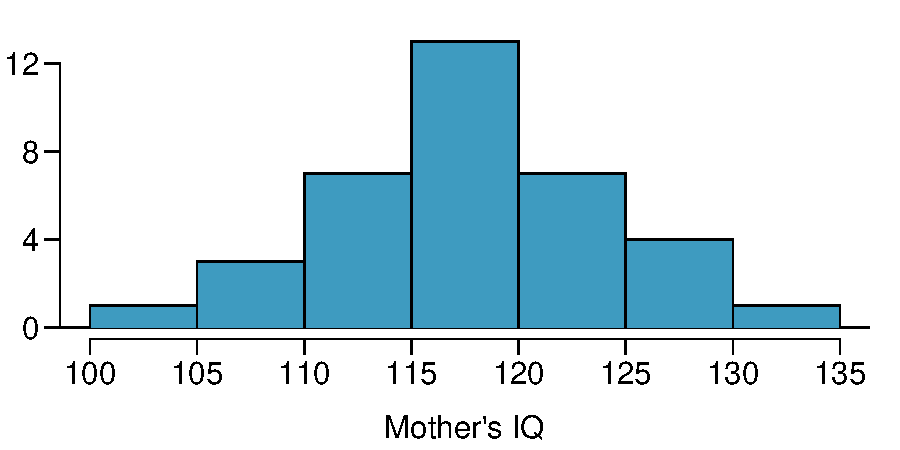
\includegraphics[width=0.94\textwidth]{ch_inference_foundations_oi_biostat/figures/eoce/gifted/gifted_momIQ_hist}
\end{center}
\end{minipage}\vspaceB{-2mm}
}{}

% 25

\eoce{\qt{Nutrition labels} The nutrition label on a bag of potato chips says that a one ounce (28 gram) serving of potato chips has 130 calories and contains ten grams of fat, with three grams of saturated fat. A random sample of 35 bags yielded a sample mean of 134 calories with a standard deviation of 17 calories. Is there evidence that the nutrition label does not provide an accurate measure of calories in the bags of potato chips? We have verified the independence, sample size, and skew conditions are satisfied.
}{}

% 26

\eoce{\qt{Find the sample mean} You are given the following hypotheses: $H_0$: $\mu = 34$, $H_A$: $\mu > 34$. We know that the sample standard deviation is 10 and the sample size is 65. For what sample mean would the p-value be equal to 0.05? Assume that all conditions necessary for inference are satisfied.
}{}

% 27

\eoce{\qt{Testing for Fibromyalgia} A patient named Diana was diagnosed with Fibromyalgia, a long-term syndrome of body pain, and was prescribed anti-depressants. Being the skeptic that she is, Diana didn't initially believe that anti-depressants would help her symptoms. However after a couple months of being on the medication she decides that the anti-depressants are working, because she feels like her symptoms are in fact getting better.
\begin{parts}
\item Write the hypotheses in words for Diana's skeptical position when she started taking the anti-depressants.
\item What is a Type 1 error in this context?
\item What is a Type 2 error in this context?
\item How would these errors affect the patient?
\end{parts}
}{}

% 28

\eoce{\qt{Testing for food safety} A food safety inspector is called upon to investigate a restaurant with a few customer reports of poor sanitation practices. The food safety inspector uses a hypothesis testing framework to evaluate whether regulations are not being met. If he decides the restaurant is in gross violation, its license to serve food will be revoked.
\begin{parts}
\item Write the hypotheses in words.
\item What is a Type 1 error in this context?
\item What is a Type 2 error in this context?
\item Which error is more problematic for the restaurant owner? Why?
\item Which error is more problematic for the diners? Why?
\item As a diner, would you prefer that the food safety inspector requires strong evidence or very strong evidence of health concerns before revoking a restaurant's license? Explain your reasoning.
\end{parts}
}{}


% 29

\eoce{\qt{Errors in drug testing} Suppose regulators monitored 403 drugs last year, each for a particular adverse response. For each drug they conducted a single hypothesis test with a significance level of 5\% to determine if the adverse effect was higher in those taking the drug than those who did not take the drug; the regulators ultimately rejected the null hypothesis for 42 drugs.
\begin{parts}
\item Describe the error the regulators might have made for a drug where the null hypothesis was rejected.
\item Describe the error regulators might have made for a drug where the null hypothesis was not rejected.
\item Suppose the vast majority of the 403 drugs do not have adverse effects. Then, if you picked one of the 42 suspect drugs at random, about how sure would you be that the drug really has an adverse effect?
\item Can you also say how sure you are that a particular drug from the 361 where the null hypothesis was not rejected does not have the corresponding adverse response?
\end{parts}
}{}

% 30

\eoce{\qt{Car insurance savings, Part I} \label{carInsurance} A car insurance company advertises that customers switching to their insurance save, on average, \$432 on their yearly premiums. A market researcher at a competing insurance discounter is interested in showing that this value is an overestimate so he can provide evidence to government regulators that the company is falsely advertising their prices. He randomly samples 82 customers who recently switched to this insurance and finds an average savings of \$395, with a standard deviation of \$102.
\begin{parts}
\item Are conditions for inference satisfied?
\item Perform a hypothesis test and state your conclusion.
\item Do you agree with the market researcher that the amount of savings advertised is an overestimate? Explain your reasoning.
\item Calculate a 90\% confidence interval for the average amount of savings of all customers who switch their insurance.
\item Do your results from the hypothesis test and the confidence interval agree? Explain.
\end{parts}
}{}

\textB{\newpage}

% 31

\eoce{\qt{Happy hour} A restaurant owner is considering extending the happy hour at his restaurant since he would like to see if it increases revenue. If it does, he will permanently extend happy hour. He estimates that the current average revenue per customer is \$18 during happy hour. He runs the extended happy hour for a week and finds an average revenue of \$19.25 with a standard deviation \$3.02 based on a simple random sample of 70 customers. \vspace{-1mm}
\begin{parts}
\item Are conditions for inference satisfied?
\item Perform a hypothesis test. Suppose the customers and their buying habits this week were no different than in any other week for this particular bar. (This may not always be a reasonable assumption.)
\item Calculate a 90\% confidence interval for the average revenue per customer.
\item Do your results from the hypothesis test and the confidence interval agree? Explain.
\item If your hypothesis test and confidence interval suggest a significant increase in revenue per customer, why might you still not recommend that the restaurant owner extend the happy hour based on this criterion? What may be a better measure to consider?
\end{parts}
}{}

% 32

\eoce{\qt{Speed reading, Part I} \label{speedReading} A company offering online speed reading courses claims that students who take their courses show a 5 times (500\%) increase in the number of words they can read in a minute without losing comprehension. A random sample of 100 students yielded an average increase of 415\% with a standard deviation of 220\%. Is there evidence that the company's claim is false?
\begin{parts}
\item Are conditions for inference satisfied?
\item Perform a hypothesis test evaluating if the company's claim is reasonable or if the true average improvement is less than 500\%. Make sure to interpret your response in context of the hypothesis test and the data. Use $\alpha = 0.025$.
\item Calculate a 95\% confidence interval for the average increase in the number of words students can read in a minute without losing comprehension.
\item Do your results from the hypothesis test and the confidence interval agree? Explain.
\end{parts}
}{}


%__________________
\subsection{Examining the Central Limit Theorem}

% 33

\eoce{\qt{Ages of pennies, Part I} \label{penniesAges} The histogram below shows the distribution of ages of pennies at a bank. 

\noindent\begin{minipage}[c]{0.5\textwidth}
\begin{parts}
\item Describe the distribution.
\item Sampling distributions for means from simple random samples of 5, 30, and 100 pennies is shown in the histograms below. Describe the shapes of these distributions and comment on whether they look like what you would expect to see based on the Central Limit Theorem.
\end{parts}\vspace{3mm}
\end{minipage}
\begin{minipage}[c]{0.5\textwidth}
\begin{center}
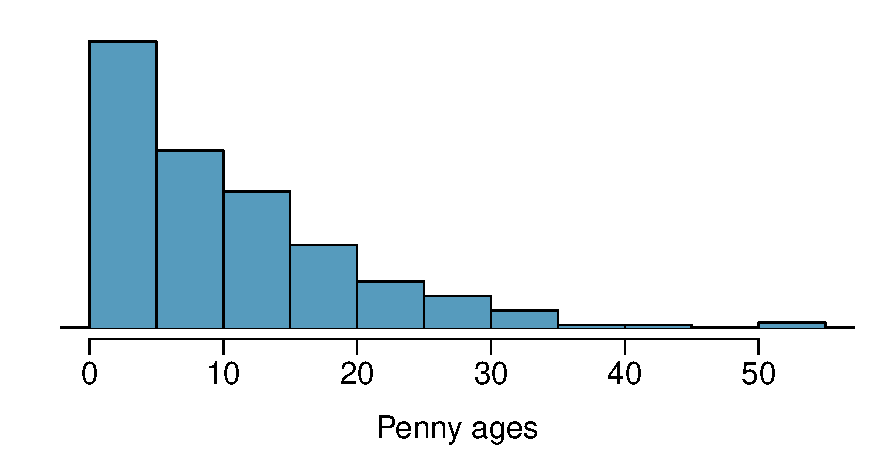
\includegraphics[width=\textwidth]{ch_inference_foundations_oi_biostat/figures/eoce/penniesAges/penniesAges_pop} 
\end{center}
\end{minipage}\vspace{-1mm}
\begin{center}
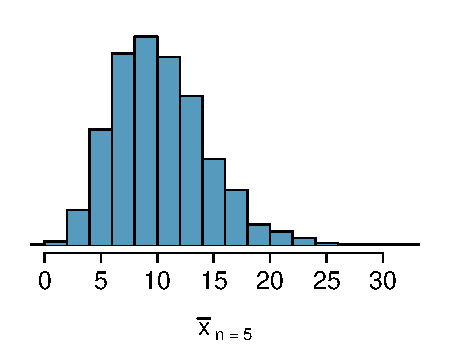
\includegraphics[width=0.325\textwidth]{ch_inference_foundations_oi_biostat/figures/eoce/penniesAges/penniesAges_n5} 
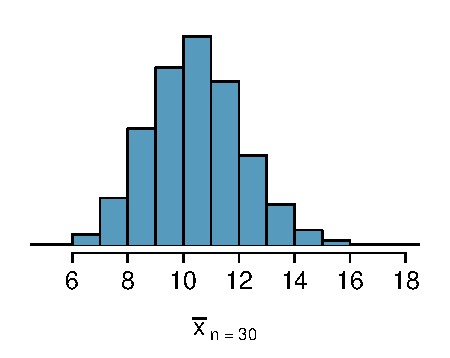
\includegraphics[width= 0.325\textwidth]{ch_inference_foundations_oi_biostat/figures/eoce/penniesAges/penniesAges_n30} 
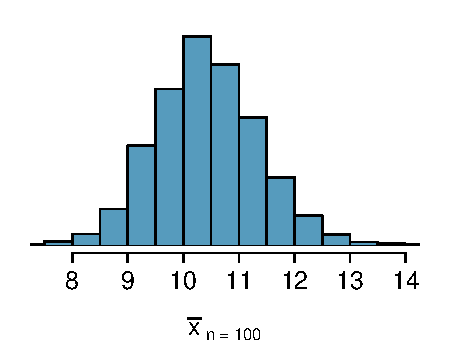
\includegraphics[width= 0.325\textwidth]{ch_inference_foundations_oi_biostat/figures/eoce/penniesAges/penniesAges_n100} 
\end{center}
}{}

% 34

\eoce{\qt{Ages of pennies, Part II} The mean age of the pennies from Exercise~\ref{penniesAges} is 10.44 years with a standard deviation of 9.2 years. Using the Central Limit Theorem, calculate the means and standard deviations of the distribution of the mean from random samples of size 5, 30, and 100. Comment on whether the sampling distributions shown in Exercise~\ref{penniesAges} agree with the values you compute.
}{}

% 35

\eoce{\qt{Identify distributions, Part I} Four plots are presented below. The plot at the top is a distribution for a population. The mean is 10 and the standard deviation is 3. Also shown below is a distribution of (1) a single random sample of 100 values from this population, (2) a distribution of 100 sample means from random samples with size 5, and (3) a distribution of 100 sample means from random samples with size 25. Determine which plot (A, B, or C) is which and explain your reasoning.
\begin{center}
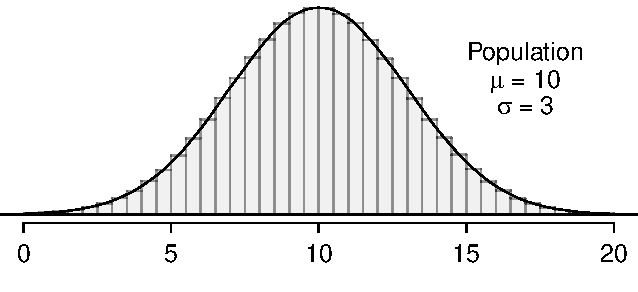
\includegraphics[width=0.5\textwidth]{ch_inference_foundations_oi_biostat/figures/eoce/cltSimSYM/cltSimSYM_pop}
\end{center}
\begin{center}
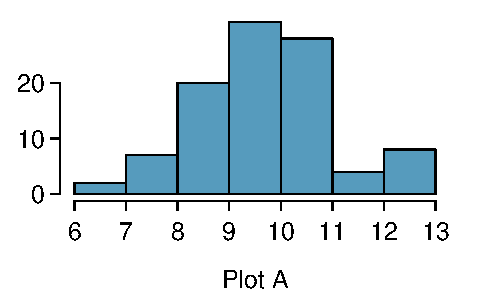
\includegraphics[width=0.32\textwidth]{ch_inference_foundations_oi_biostat/figures/eoce/cltSimSYM/cltSimSYM_n5}
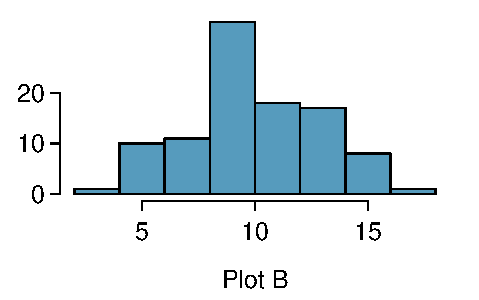
\includegraphics[width=0.32\textwidth]{ch_inference_foundations_oi_biostat/figures/eoce/cltSimSYM/cltSimSYM_samp}
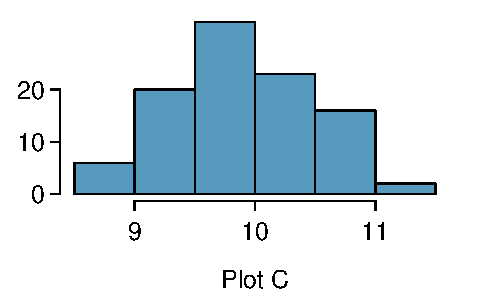
\includegraphics[width=0.32\textwidth]{ch_inference_foundations_oi_biostat/figures/eoce/cltSimSYM/cltSimSYM_n25}
\end{center}
}{}

% 36

\eoce{\qt{Identify distributions, Part II} Four plots are presented below. The plot at the top is a distribution for a population. The mean is 60 and the standard deviation is 18. Also shown below is a distribution of (1) a single random sample of 500 values from this population, (2) a distribution of 500 sample means from random samples of each size 18, and (3) a distribution of 500 sample means from random samples of each size 81. Determine which plot (A, B, or C) is which and explain your reasoning.
\begin{center}
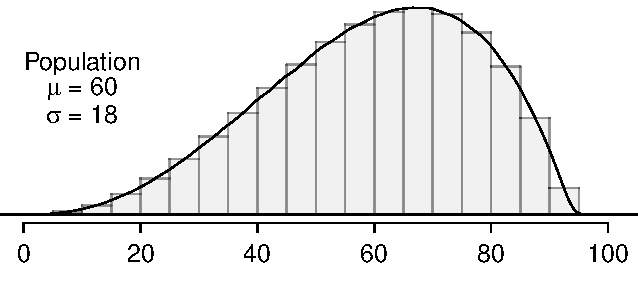
\includegraphics[width=0.5\textwidth]{ch_inference_foundations_oi_biostat/figures/eoce/cltSimLS/cltSimLS_pop}
\end{center}
\begin{center}
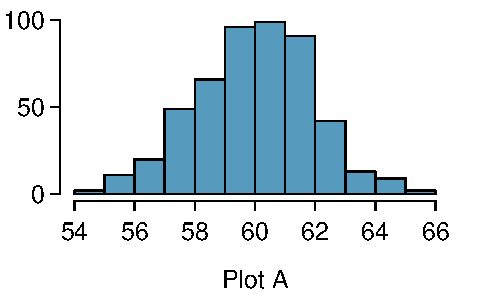
\includegraphics[width=0.32\textwidth]{ch_inference_foundations_oi_biostat/figures/eoce/cltSimLS/cltSimLS_n81}
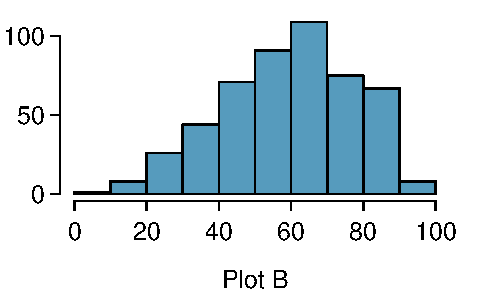
\includegraphics[width=0.32\textwidth]{ch_inference_foundations_oi_biostat/figures/eoce/cltSimLS/cltSimLS_samp}
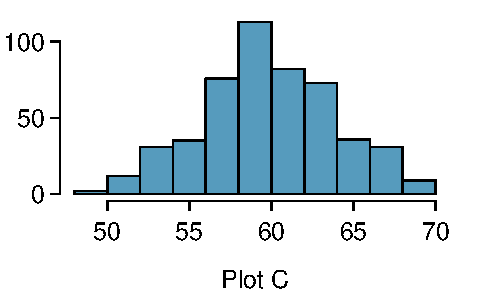
\includegraphics[width=0.32\textwidth]{ch_inference_foundations_oi_biostat/figures/eoce/cltSimLS/cltSimLS_n18}
\end{center}
}{} 

% 37

\eoce{\qt{Housing prices, Part I} \label{Topanga} A housing survey was conducted to determine the price of a typical home in Topanga, CA. The mean price of a house was roughly \$1.3 million with a standard deviation of \$300,000. There were no houses listed below \$600,000 but a few houses above \$3 million.
\begin{parts}
\item Is the distribution of housing prices in Topanga symmetric, right skewed, or left skewed? \textit{Hint:} Sketch the distribution.
\item Would you expect most houses in Topanga to cost more or less than \$1.3 million?
\item Can we estimate the probability that a randomly chosen house in Topanga costs more than \$1.4 million using the normal distribution?
\item What is the probability that the mean of 60 randomly chosen houses in Topanga is more than \$1.4 million?
\item How would doubling the sample size affect the standard error of the mean?
\end{parts}
}{}

% 38

\eoce{\qt{Stats final scores} Each year about 1500 students take the introductory statistics course at a large university. This year scores on the final exam are distributed with a median of 74 points, a mean of 70 points, and a standard deviation of 10 points. There are no students who scored above 100 (the maximum score attainable on the final) but a few students scored below 20 points.
\begin{parts}
\item Is the distribution of scores on this final exam symmetric, right skewed, or left skewed?
\item Would you expect most students to have scored above or below 70 points?
\item Can we calculate the probability that a randomly chosen student scored above 75 using the normal distribution?
\item What is the probability that the average score for a random sample of 40 students is above 75?
\item How would cutting the sample size in half affect the standard error of the mean?
\end{parts}
}{}

% 39

\eoce{\qt{Weights of pennies} The distribution of weights of US pennies is approximately normal with a mean of 2.5 grams and a standard deviation of 0.03 grams.
\begin{parts}
\item What is the probability that a randomly chosen penny weighs less than 2.4 grams?
\item Describe the sampling distribution of the mean weight of 10 randomly chosen pennies.
\item What is the probability that the mean weight of 10 pennies is less than 2.4 grams?
\item Sketch the two distributions (population and sampling) on the same scale.
\item Could you estimate the probabilities from (a) and (c) if the weights of pennies had a skewed distribution?
\end{parts}
}{}

% 40

\eoce{\qt{CFLs} A manufacturer of compact fluorescent light bulbs advertises that the distribution of the lifespans of these light bulbs is nearly normal with a mean of 9,000 hours and a standard deviation of 1,000 hours.
\begin{parts}
\item What is the probability that a randomly chosen light bulb lasts more than 10,500 hours?
\item Describe the distribution of the mean lifespan of 15 light bulbs. 
\item What is the probability that the mean lifespan of 15 randomly chosen light bulbs is more than 10,500 hours?
\item Sketch the two distributions (population and sampling) on the same scale.
\item Could you estimate the probabilities from parts~(a) and~(c) if the lifespans of light bulbs had a skewed distribution?
\end{parts}
}{}

\textB{\newpage}

% 41

\eoce{\qt{Songs on an  iPod} Suppose an iPod has 3,000 songs. The histogram below shows the distribution of the lengths of these songs. We also know that, for this iPod, the mean length is 3.45 minutes and the standard deviation is 1.63 minutes. 
\begin{center}
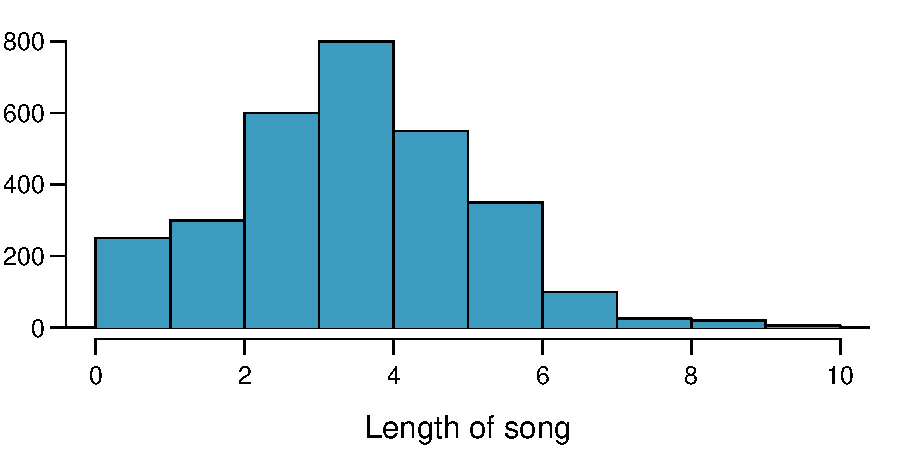
\includegraphics[width=0.75\textwidth]{ch_inference_foundations_oi_biostat/figures/eoce/ipod/ipod_popdist}
\end{center}
\begin{parts}
\item Calculate the probability that a randomly selected song lasts more than 5 minutes.
\item You are about to go for an hour run and you make a random playlist of 15 songs. What is the probability that your playlist lasts for the entire duration of your run? \textit{Hint:} If you want the playlist to last 60 minutes, what should be the minimum average length of a song?
\item You are about to take a trip to visit your parents and the drive is 6 hours. You make a random playlist of 100 songs. What is the probability that your playlist lasts the entire drive?
\end{parts}
}{}

% 42

\eoce{\qt{Spray paint} Suppose the area that can be painted using a single can of spray paint is slightly variable and follows a nearly normal distribution with a mean of 25 square feet and a standard deviation of 3 square feet. 
\begin{parts}
\item What is the probability that the area covered by a can of spray paint is more than 27 square feet?
\item Suppose you want to spray paint an area of 540 square feet using 20 cans of spray paint. On average, how many square feet must each can be able to cover to spray paint all 540 square feet?
\item What is the probability that you can cover a 540 square feet area using 20 cans of spray paint?
\item If the area covered by a can of spray paint had a slightly skewed distribution, could you still calculate the probabilities in parts~(a) and~(c) using the normal distribution?
\end{parts}
}{}


\textB{\newpage}

%__________________
\subsection{Inference for other estimators}

% 43

\eoce{\qt{Spam mail, Part I} \label{spam} The 2004 National Technology Readiness Survey sponsored by the Smith School of Business at the University of Maryland surveyed 418 randomly sampled Americans, asking them how many spam emails they receive per day. The survey was repeated on a new random sample of 499 Americans in 2009.\footfullcite{webpage:spam}
\begin{parts}
\item What are the hypotheses for evaluating if the average spam emails per day has changed from 2004 to 2009.
\item In 2004 the mean was 18.5 spam emails per day, and in 2009 this value was 14.9 emails per day. What is the point estimate for the difference between the two population means?
\item A report on the survey states that the observed difference between the sample means is not statistically significant. Explain what this means in context of the hypothesis test and the data.
\item Would you expect a confidence interval for the difference between the two population means to contain 0? Explain your reasoning.
\end{parts}
}{}

% 44

\eoce{\qt{Nearsightedness} It is believed that nearsightedness affects about 8\% of all children. In a random sample of 194 children, 21 are nearsighted.
\begin{parts}
\item Construct hypotheses appropriate for the following question: do these data provide evidence that the 8\% value is inaccurate?
\item What proportion of children in this sample are nearsighted?
\item Given that the standard error of the sample proportion is 0.0195 and the point estimate follows a nearly normal distribution, calculate the test statistic (the Z statistic).
\item What is the p-value for this hypothesis test?
\item What is the conclusion of the hypothesis test?
\end{parts}
}{}

% 45

\eoce{\qt{Spam mail, Part II} The National Technology Readiness Survey from Exercise~\ref{spam} also asked Americans how often they delete spam emails. 23\% of the respondents in 2004 said they delete their spam mail once a month or less, and in 2009 this value was 16\%.
\begin{parts}
\item What are the hypotheses for evaluating if the proportion of those who delete their email once a month or less (or never) has changed from 2004 to 2009?
\item What is the point estimate for the difference between the two population proportions?
\item A report on the survey states that the observed decrease from 2004 to 2009 is statistically significant. Explain what this means in context of the hypothesis test and the data.
\item Would you expect a confidence interval for the difference between the two population proportions to contain 0? Explain your reasoning.
\end{parts}
}{}

% 46

\eoce{\qt{Unemployment and relationship problems} A USA Today/Gallup poll conducted between 2010 and 2011 asked a group of unemployed and underemployed Americans if they have had major problems in their relationships with their spouse or another close family member as a result of not having a job (if unemployed) or not having a full-time job (if underemployed). 27\% of the 1,145 unemployed respondents and 25\% of the 675 underemployed respondents said they had major problems in relationships as a result of their employment status.
\begin{parts}
\item What are the hypotheses for evaluating if the proportions of unemployed and underemployed people who had relationship problems were different?
\item The p-value for this hypothesis test is approximately 0.35. Explain what this means in context of the hypothesis test and the data.
\end{parts}
}{}

\textB{\newpage}


%__________________
\subsection{Sample size and power}

% 47

\eoce{\qtq{Which is higher} In each part below, there is a value of interest and two scenarios (I and II). For each part, report if the value of interest is larger under scenario I, scenario II, or whether the value is equal under the scenarios.
\begin{parts}
\item The standard error of $\bar{x}$ when $s = 120$ and (I) n = 25 or (II) n = 125.
\item The margin of error of a confidence interval when the confidence level is (I) 90\% or (II) 80\%.
\item The p-value for a Z statistic of 2.5 when (I) n = 500 or (II) n = 1000.
\item The probability of making a Type 2 error when the alternative hypothesis is true and the significance level is (I) 0.05 or (II) 0.10.
\end{parts}
}{}

% 48

\eoce{\qt{True or false} Determine if the following statements are true or false, and explain your reasoning. If false, state how it could be corrected.
\begin{parts}
\item If a given value (for example, the null hypothesized value of a parameter) is within a 95\% confidence interval, it will also be within a 99\% confidence interval.
\item Decreasing the significance level ($\alpha$) will increase the probability of making a Type 1 error.
\item Suppose the null hypothesis is $\mu = 5$ and we fail to reject $H_0$. Under this scenario, the true population mean is 5.
\item If the alternative hypothesis is true, then the probability of making a Type 2 error and the power of a test add up to 1.
\item With large sample sizes, even small differences between the null value and the true value of the parameter, a difference often called the effect size\index{effect size}, will be identified as statistically significant.
\item A cutoff of $\alpha$ = 0.05 is the ideal value for all hypothesis tests.
\end{parts}
}{}

% 49

\eoce{\qt{Car insurance savings, Part II} The market researcher from Exercise~\ref{carInsurance} collected data about the savings of 82 customers at a competing car insurance company. The mean and standard deviation of this sample are \$395 and \$102, respectively. He would like to conduct another survey but have a margin of error of  no more than \$10 at a 99\% confidence level. How large of a sample should he collect?
}{}

% 50

\eoce{\qt{Speed reading, Part II} A random sample of 100 students who took online speed reading courses from the company described in Exercise~\ref{speedReading} yielded an average increase in reading speed of 415\% and a standard deviation of 220\%. We would like to calculate a 95\% confidence interval for the average increase in reading speed with a margin of error of no more than 15\%. How many students should we sample?
}{}

% 51

\eoce{\qt{Waiting at the ER, Part IV} Exercise~\ref{ERWaitHT} introduced us to a hospital where ER wait times were being analyzed. The previous year's average was 128 minutes. Suppose that this year's average wait time is 135 minutes.
\begin{parts}
\item Provide the hypotheses for this situation in plain language.
\item If we plan to collect a sample size of $n=64$, what values could $\bar{x}$ take so that we reject $H_0$? Suppose the sample standard deviation from the earlier exercise (39 minutes) is the population standard deviation. You may assume that the conditions for the nearly normal model for $\bar{x}$ are satisfied.
\item Calculate the probability of a Type 2 error.
\end{parts}
}{}
